\chapter{Metodologia}

A metodologia concebida para a realização deste trabalho foi classificada quanto à sua natureza, abordagem e aos procedimentos técnicos.

Quanto à natureza, a pesquisa possui uma caracterização aplicada, visto que se objetiva gerar conhecimentos de efeito prático e destinados à resolução de problemas específicos. Quanto à abordagem, a pesquisa possui um enfoque qualitativo, devido ao fato de não requerer a utilização de métodos e técnicas estatísticas \cite{metodologia}.

Para concretizar a realização do trabalho, os seguintes procedimentos técnicos foram adotados:

\begin{itemize}
	\item Pesquisa Bibliográfica
	\item Revisão Sistemática
\end{itemize}

Pelo fato de o presente trabalho estar centrado na proposição de um \textit{framework} que reúne práticas propostas pela verificação de \textit{software} e integra estas às diretrizes fornecidas pela VBSE, fez-se necessária a seleção de mais de um procedimento técnico de pesquisa para a construção do trabalho.
 
O arcabouço teórico inerente à VBSE e às inspeções de código foi obtido a partir da pesquisa bibliográfica.

Para Fonseca (2002), a pesquisa bibliográfica é realizada a partir do levantamento de referências teóricas já analisadas, e publicadas por meios escritos e eletrônicos. A pesquisa bibliográfica possibilita que o pesquisador conheça o que já se estudou sobre a temática.

A revisão sistemática, por sua vez, se estabelece como uma metodologia bem definida para identificar, analisar e interpretar as melhores abordagens e práticas relacionadas à uma determinada questão de pesquisa \cite{sistematica}. Além desses aspectos, é uma metodologia que possibilita uma repetição concisa.

A opção pelo procedimento da revisão sistemática deve-se ao fato de que este trabalho também está voltado para a tentativa de compreender quais tem sido as abordagens empregadas na elaboração de testes unitários e como se tem avaliado a efetividade destes. O \textit{framework}, naturalmente, compreende a prática de elaboração de testes unitários.

Outro aspecto interessante da revisão sistemática é que esta auxilia de maneira precisa na localização dos principais trabalhos publicados para uma determinada problemática, favorecendo a construção de uma linha cronológica que demonstra ao pesquisador quais linhas têm sido defendidas e quais são os campos mais promissores para uma futura exploração.

Neste trabalho, para a execução da revisão sistemática, considerou-se a proposta de Kitchenham para a revisão no âmbito da Engenharia de \textit{Software}. A proposta é composta por três fases:

\begin{itemize}
	\item Planejamento da revisão
	\item Condução da revisão
	\item Relato da revisão
\end{itemize}

A fase de planejamento consiste na identificação da necessidade de se desenvolver uma revisão sistemática, bem como elaborar um protocolo de revisão. Logo em seguida, na fase de condução, os objetivos mais pontuais de pesquisa são identificados e, adicionalmente, estudos são selecionados e seus dados são extraídos e analisados. Por fim, na fase de relato, os dados extraídos e analisados na fase anterior são externalisados e elabora-se uma discussão. Maiores detalhes acerca da revisão sistemática executada neste trabalho podem ser encontrados no Apêndice A.

\section{Detalhamento do Plano Metodológico}

O plano metodológico concebido para a formulação e aplicação do \textit{framework} aqui proposto se subdivide em duas partes, sendo a primeira atrelada ao TCC 1 (Trabalho de Conclusão de Curso 1) e a segunda, ao TCC 2.

A primeira parte compreende 3 fases: \textit{Planejamento da Pesquisa}; \textit{Coleta de Informações} e \textit{Proposta de Solução}.

A fase inerente ao \textit{Planejamento da Pesquisa} envolve a definição de objetivos, pergunta de pesquisa, classificação metodológica e estabelecimento dos procedimentos técnicos de pesquisa. É válido evidenciar que essas definições são realizadas a partir do problema que foi identificado.

A fase de \textit{Coleta de Informações} compreende a aplicação dos procedimentos técnicos adotados para a pesquisa, que para este trabalho foram a pesquisa bibliográfica e a revisão sistemática.

Por fim, na fase \textit{Proposta de Solução}, há a concepção de uma possível solução para a problemática identificada. Esta solução, por sua vez, está embasada nas informações coletadas na fase anterior.

A figura a seguir ilustra essa parte do plano metodológico.

\begin{figure}[h]
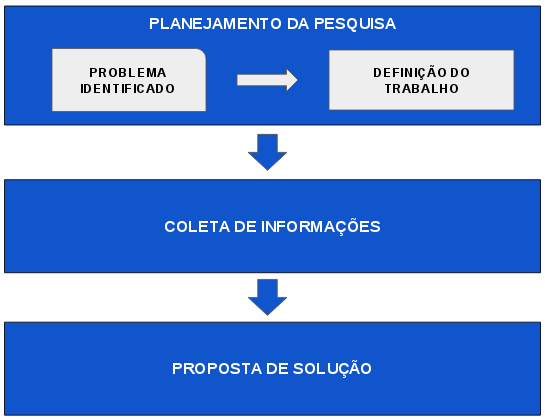
\includegraphics[width=\textwidth]{figuras/planometodologico1.png}
\caption{Plano Metodológico - TCC 1}
\end{figure}

A segunda parte, já vinculada ao TCC 2, envolve outras 3 fases: \textit{Coleta de Dados}; \textit{Análise e Interpretação dos Resultados} e \textit{Divulgação dos Resultados.}.
A fase \textit{Coleta de Dados} envolve a aplicação de um procedimento técnico denominado pesquisa-ação. Esse procedimento possibilita que o pesquisador intervenha dentro da problemática, mobilizando os participantes e construindo novos conhecimentos \cite{pesquisa}. Assim, a cada ciclo novos quesitos poderão ser melhor tratados no \textit{framework}.

Na fase \textit{Análise e Interpretação dos Resultados}, todos os dados coletados a partir da utilização do \textit{framework} serão analisados, de forma que todas as percepções possíveis possam ser obtidas. Por fim, na fase \textit{Divulgação dos Resultados}, haverá uma estruturação de todos os dados obtidos e analisados, de forma que possa ser evidenciado a efetividade do uso do \textit{framework}.

A figura a seguir ilustra a segunda parte do plano metodológico.

\begin{figure}[h]
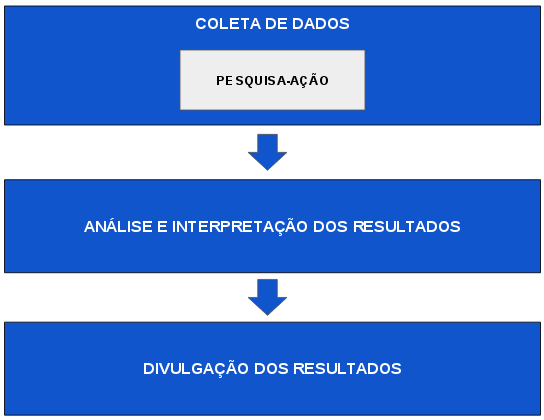
\includegraphics[width=\textwidth]{figuras/planometodologico2.png}
\caption{Plano Metodológico - TCC 2}
\end{figure}